\documentclass[../../main.tex]{subfiles}

\begin{document}

	\subsection{Reliability}

	CLup's queueing system is critical in order to keep track of the accesses, thus its infrastructure 
	should be characterized by the highest MTTF and lowest MTTR possible.

	A larger MTTR is acceptable for the other services, however it's mandatory to ensure the lack of 
	data losses during downtime.

	\subsection{Availability}

	All services must be up and running 24/7, both supermarkets and users need to be notified in case of 
	any communication issues with CLup servers.

	Stores should be able to communicate with CLup's servers during all their opening time span.

	As shown in the following histogram, it is expected an high utilisation of all services during the day, 
	and a low usage during night hours.

	\begin{figure}[h!]
	    \centering
	    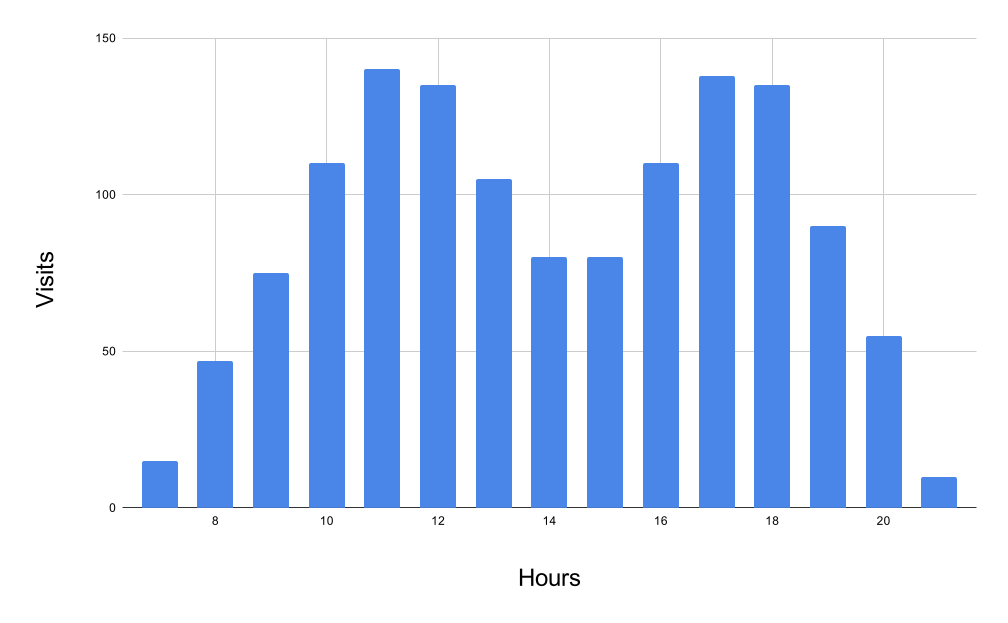
\includegraphics[width=0.8\textwidth]{affluence-chart.png}
	    \caption{Average daily visits in the biggest supermarket in Milan. \\Credits: Google.}
  	\end{figure}

	\subsection{Security}

	All data inbound to CLup services must be treated as stated by security regulations. 

	To maximise security in the authentication phases, the system should use OAuth 2.0 authorisation framework.

	Additionally, in order to guarantee the protection of the customer's data in between servers and the 
	user's device, all Internet traffic must be encrypted with SSL, and sent via HTTPS protocol.

	To enhance server-side security, passwords must always be hashed to protect the system or minimize the damage 
	in case of Cyber-Attacks. 

	\subsection{Maintainability}

	\subsection{Portability}

	
\end{document}